%%%%%%%%%%%%%%%%%%%%%%%%%%%%%%%%%%%%%%%%%
% Jacobs Landscape Poster
% LaTeX Template
% Version 1.0 (29/03/13)
%
% Created by:
% Computational Physics and Biophysics Group, Jacobs University
% https://teamwork.jacobs-university.de:8443/confluence/display/CoPandBiG/LaTeX+Poster
% 
% Further modified by:
% Nathaniel Johnston (nathaniel@njohnston.ca)
%
% This template has been downloaded from:
% http://www.LaTeXTemplates.com
%
% License:
% CC BY-NC-SA 3.0 (http://creativecommons.org/licenses/by-nc-sa/3.0/)
%
%%%%%%%%%%%%%%%%%%%%%%%%%%%%%%%%%%%%%%%%%

%----------------------------------------------------------------------------------------
%   PACKAGES AND OTHER DOCUMENT CONFIGURATIONS
%----------------------------------------------------------------------------------------

\documentclass[final]{beamer}

\usepackage[scale=1.24]{beamerposter} % Use the beamerposter package for laying out the poster

\usetheme{confposter} % Use the confposter theme supplied with this template

\setbeamercolor{block title}{fg=ngreen,bg=white} % Colors of the block titles
\setbeamercolor{block body}{fg=black,bg=white} % Colors of the body of blocks
\setbeamercolor{block alerted title}{fg=white,bg=dblue!70} % Colors of the highlighted block titles
\setbeamercolor{block alerted body}{fg=black,bg=dblue!10} % Colors of the body of highlighted blocks
% Many more colors are available for use in beamerthemeconfposter.sty

%-----------------------------------------------------------
% Define the column widths and overall poster size
% To set effective sepwid, onecolwid and twocolwid values, first choose how many columns you want and how much separation you want between columns
% In this template, the separation width chosen is 0.024 of the paper width and a 4-column layout
% onecolwid should therefore be (1-(# of columns+1)*sepwid)/# of columns e.g. (1-(4+1)*0.024)/4 = 0.22
% Set twocolwid to be (2*onecolwid)+sepwid = 0.464
% Set threecolwid to be (3*onecolwid)+2*sepwid = 0.708

\newlength{\sepwid}
\newlength{\onecolwid}
\newlength{\twocolwid}
\newlength{\threecolwid}
\setlength{\paperwidth}{48in} % A0 width: 46.8in
\setlength{\paperheight}{40in} % A0 height: 33.1in
\setlength{\sepwid}{0.024\paperwidth} % Separation width (white space) between columns
\setlength{\onecolwid}{0.22\paperwidth} % Width of one column
\setlength{\twocolwid}{0.464\paperwidth} % Width of two columns
\setlength{\threecolwid}{0.708\paperwidth} % Width of three columns
\setlength{\topmargin}{-0.5in} % Reduce the top margin size
%-----------------------------------------------------------

% \renewcommand{\sfdefault}{phv}
% \renewcommand{\rmdefault}{ptm}


\usepackage{graphicx}  % Required for including images

\usepackage{booktabs} % Top and bottom rules for tables

%----------------------------------------------------------------------------------------
%   TITLE SECTION 
%----------------------------------------------------------------------------------------

\title{The influence of the Southland Current on the circulation within Pegasus Bay} % Poster title

\author{Rafael Soutelino and Brett Beamsley} % Author(s)

\institute{MetOcean Solutions} % Institution(s)

%----------------------------------------------------------------------------------------

\begin{document}

\addtobeamertemplate{block end}{}{\vspace*{2ex}} % White space under blocks
\addtobeamertemplate{block alerted end}{}{\vspace*{2ex}} % White space under highlighted (alert) blocks

\setlength{\belowcaptionskip}{2ex} % White space under figures
\setlength\belowdisplayshortskip{2ex} % White space under equations

\begin{frame}[t] % The whole poster is enclosed in one beamer frame

\begin{columns}[t] % The whole poster consists of three major columns, the second of which is split into two columns twice - the [t] option aligns each column's content to the top

\begin{column}{\sepwid}\end{column} % Empty spacer column

\begin{column}{\onecolwid} % The first column

    %----------------------------------------------------------------------------------------
    %   OBJECTIVES
    %----------------------------------------------------------------------------------------

    \begin{alertblock}{Objectives}

    Investigate the effect of the Southland Current (SC) on the coastal circulation at Pegasus Bay (PB) using a combination of long term realistic modelling and {\it in situ} measurements.

    \begin{enumerate}
    \item What is the contribution of the SC to the total currents on the inner shelf of PB?
    \item What is the impact of remote forcing in modelling efforts at the inner shelf of PB?
    \item What are the implications of underestimating the SC flow in the prediction of arbitrary passive tracers transport and dispersion in PB?
    \end{enumerate}

    \end{alertblock}

    %----------------------------------------------------------------------------------------
    %   INTRODUCTION
    %----------------------------------------------------------------------------------------

    \begin{block}{Introduction}

    The East coast of New Zealand is a notably complex area in terms of interaction between oceanic and coastal circulation, due to the existence of important western boundary current systems flowing along the continental slopes and outer shelves (Jannelle \& Flemming, 2005). The SC is a northward/northeast-ward oceanic current that extends from Stewart Island in the south to the Chatham Rise in the north, formed at the subtropical convergence west of New Zealand (Chiswell, 1996). Most of it bends offshore towards the Chatham Rise (Figure \ref{schematics}), but a small portion bends towards PB, in the form of an anticyclonic eddy around BP (Carter \& Herzer, 1979). A net southerly alongshore depth-averaged transport is reported in previous work, potentially associated with an eddy in PB. 
    \begin{figure}
    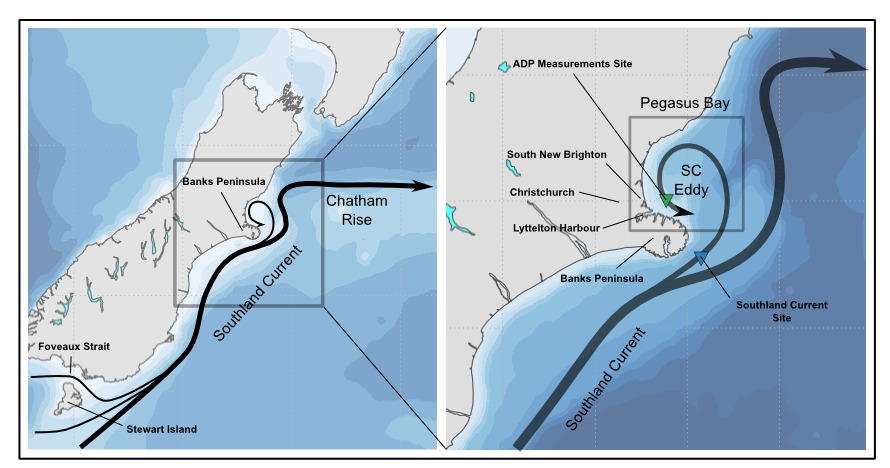
\includegraphics[width=1.0\linewidth]{schematics.png}
    \caption{\label{schematics} Circulation features off the east coast of New Zealand South Island. The green mark is the location of the observations. The blue mark is an arbitrary location within the SC path.}
    \end{figure}


    \end{block}

    \vspace{3.2cm}
    %------------------------------------------------
    % \begin{center}
    
\includegraphics[width=0.9\linewidth]{metoceanview2.jpg}
    % \end{center}

    %----------------------------------------------------------------------------------------

\end{column} % End of the first column

\begin{column}{\sepwid}\end{column} % Empty spacer column

\begin{column}{\twocolwid} % Begin a column which is two columns wide (column 2)

    \begin{columns}[t,totalwidth=\twocolwid] % Split up the two columns wide column

        \begin{column}{\onecolwid}\vspace{-.6in} % The first column within column 2 (column 2.1)

            %----------------------------------------------------------------------------------------
            %   MATERIALS
            %----------------------------------------------------------------------------------------

            \begin{block}{Methods}

            A calibrated 10-year ROMS hindcast was carried out. Two different runs were undertaken. A CONTROL run consisted of full realistic hydrodynamical forcing (Figure \ref{domains} and Table \ref{roms_configs}) and a TEST run was deprived of most of the SC incoming flow (Table \ref{experiments}).  

            \begin{figure}
            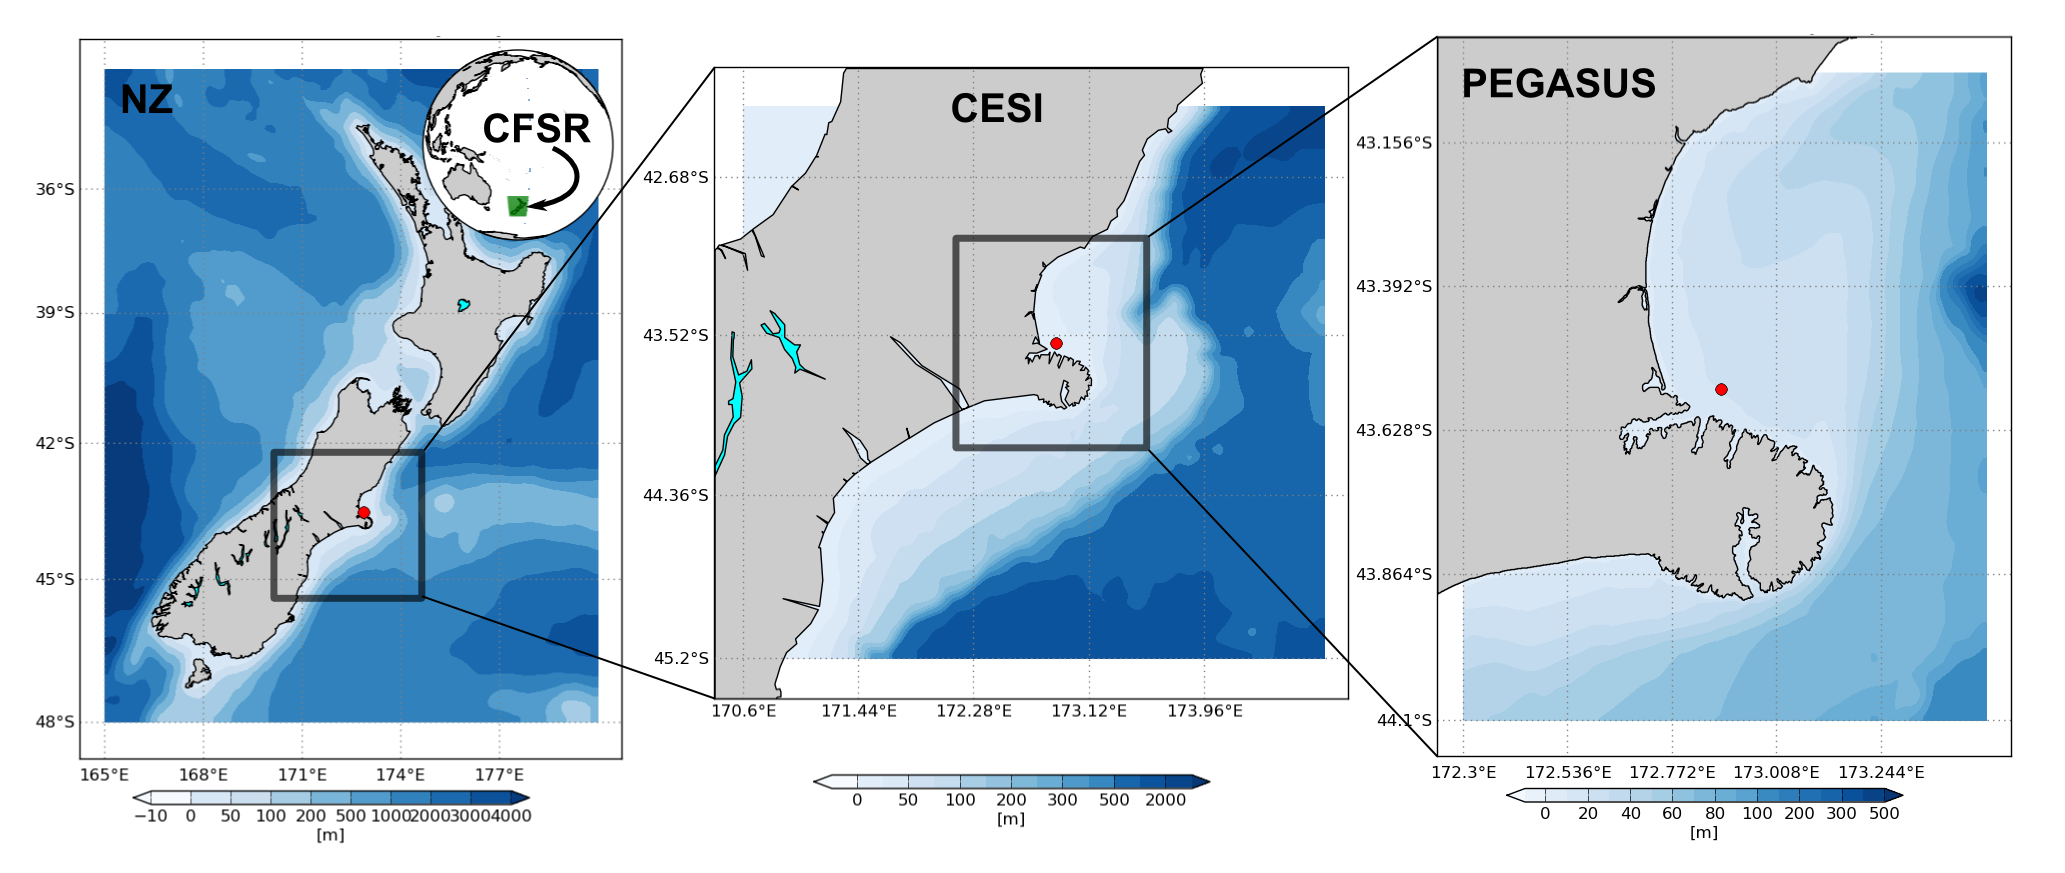
\includegraphics[width=1.0\linewidth]{domains.png}
            \caption{\label{domains} Hindcast nesting approach with ROMS. See Tables \ref{experiments} and \ref{roms_configs} for more details.}
            \end{figure}

            \begin{small}

            \begin{table}
            \vspace{2ex}
            \begin{tabular}{l c}
            \toprule
            \textbf{Experiment} & \textbf{Nests} \\
            \midrule
            \textbf{CONTROL} & CFSR $\rightarrow$ NZ $\rightarrow$ CESI $\rightarrow$ PEGASUS \\
            \textbf{TEST}    & CFSR $\rightarrow$ PEGASUS \\
            \bottomrule
            \end{tabular}
            \caption{\label{experiments} Description of the numerical experiments.}
            \end{table}


            \begin{table}
            \vspace{2ex}
            \begin{tabular}{l c c c}
            \toprule
                                & \textbf{NZ}  & \textbf{CESI} & \textbf{PEGASUS} \\
            \midrule
            \textbf{Resolution} & 0.08$^\circ$ & 0.03$^\circ$ & 0.004$^\circ$ \\
            \textbf{Boundary}   & CFSR         & NZ           & CESI          \\
            \textbf{Tides}      & No           & No           & Yes           \\
            \textbf{Meteo}      & WRF12km      & WRF12km      & WRF12km        \\
            \bottomrule
            \end{tabular}
            \caption{\label{roms_configs} ROMS domains configuration summary.}
            \end{table}

            \end{small}


            \end{block}

            \begin{block}{Results}

            As seen in Figure \ref{mean_flow}, the northeasterly flowing SC clearly bifurcates after crossing the 44.42$^\circ$ S parallel. Some of the water recirculates into PB in the form of an anticyclonic eddy. There is a clear difference in the magnitude of the mean currents predicted by the different runs. The average flow from CONTROL explained 80\% of the observations, while TEST, only 33\%. 

            \end{block}

            %----------------------------------------------------------------------------------------

        \end{column} % End of column 2.1

        \begin{column}{\onecolwid}\vspace{-.6in} % The second column within column 2 (column 2.2)

            \begin{block}

            \begin{figure}
            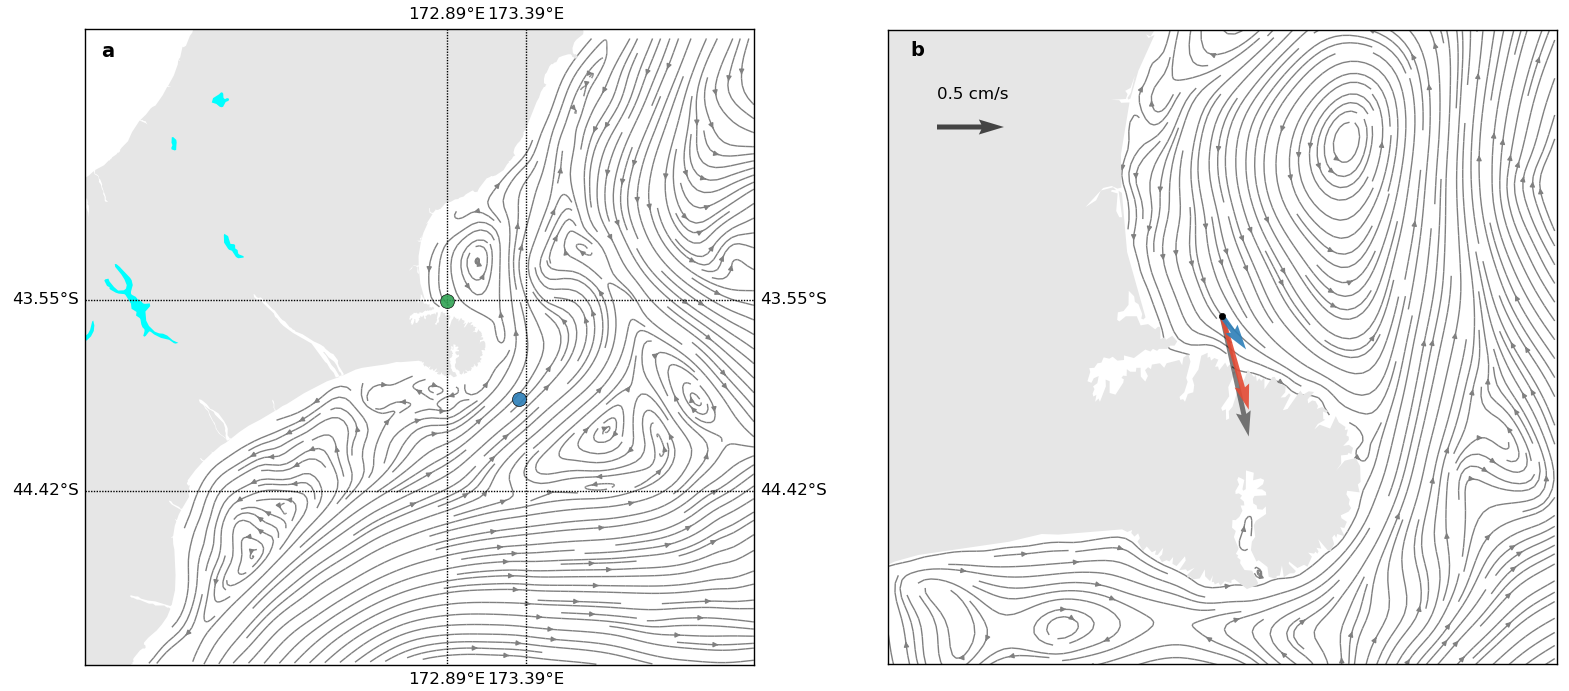
\includegraphics[width=1.0\linewidth]{mean_flow.png}
            \caption{\label{mean_flow} Feb 2008 monthly mean depth-averaged stream lines for the CESI (a) and PEGASUS (b) ROMS domains. The arrows in (b) represents the average currents from the observations (gray), the CONTROL (red) and TEST (blue) simulations.}
            \end{figure}

            According to Figure \ref{validation}, CONTROL shows good skill in reproducing the total currents. The residual currents are notably matched by the model for most events. TEST, however, produced relatively poor results. A 20 h lag between perturbations in the SC and PB (Figure \ref{spectra}) seems to occur. The spectra confirms the variability match at time scales of western boundary current variability between both locations, corroborating a clear influence of the SC in the PB circulation. 

            \begin{figure}
            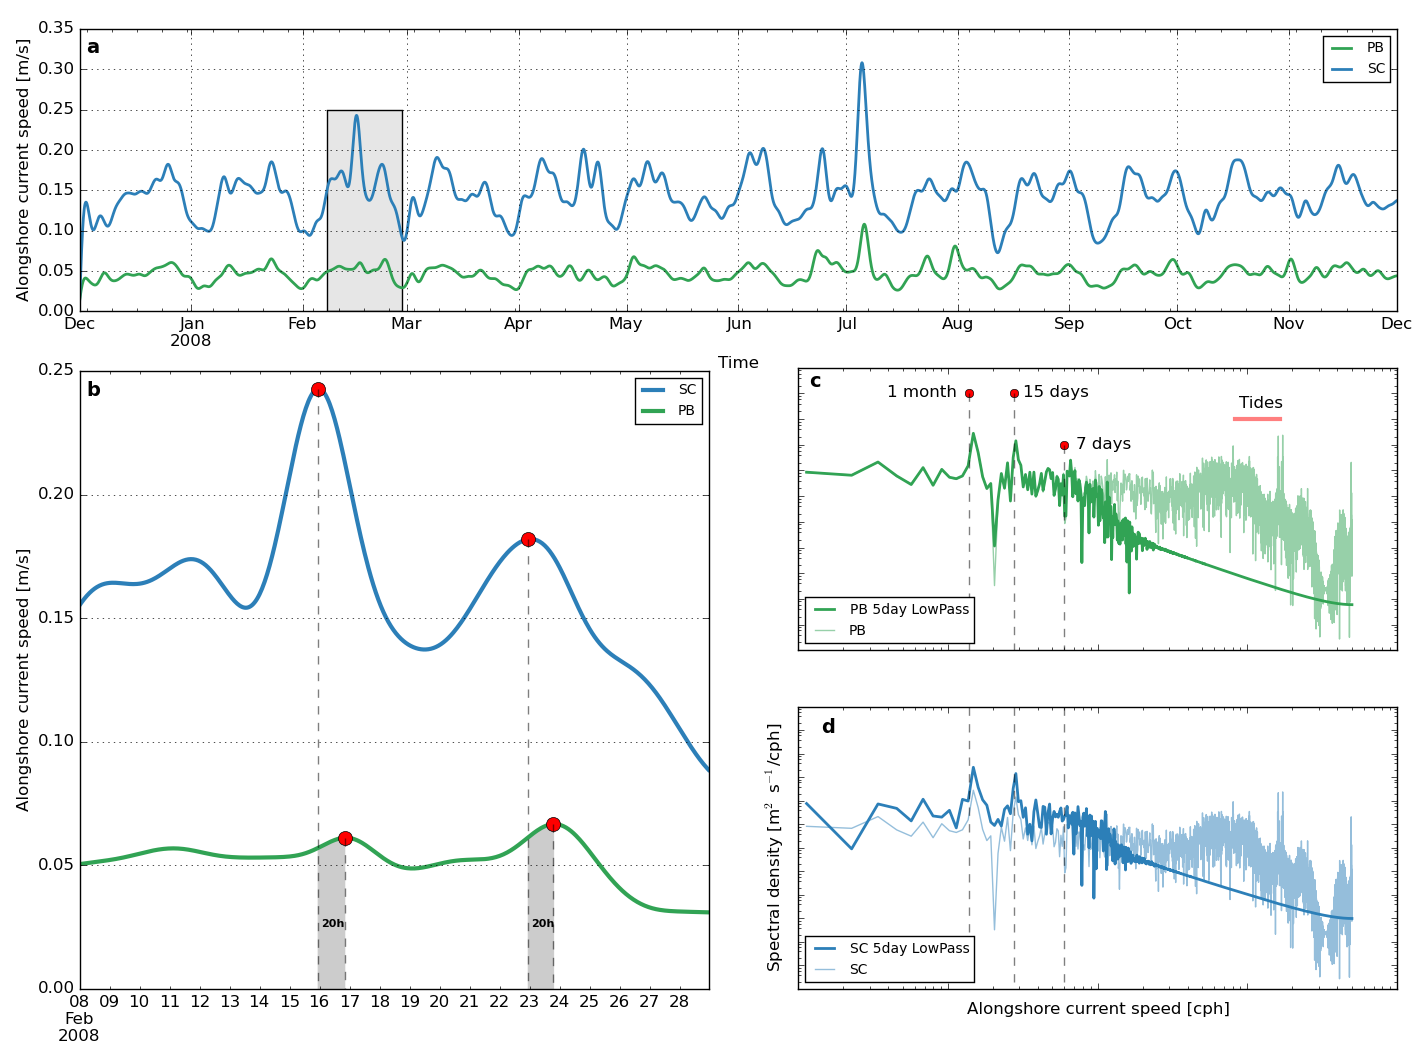
\includegraphics[width=1.0\linewidth]{pb-sc_5day-lowpass_time-series.png}
            \caption{\label{spectra} Along shore current variability analysis of the CONTROL simulation. The blue and green locations are shown in Figure \ref{mean_flow}a, with the same color coding. }
            \end{figure}

            \end{block}

            %----------------------------------------------------------------------------------------

        \end{column} % End of column 2.2

    \end{columns} % End of the split of column 2 - any content after this will now take up 2 columns width

    % \begin{block}

    \begin{figure}
    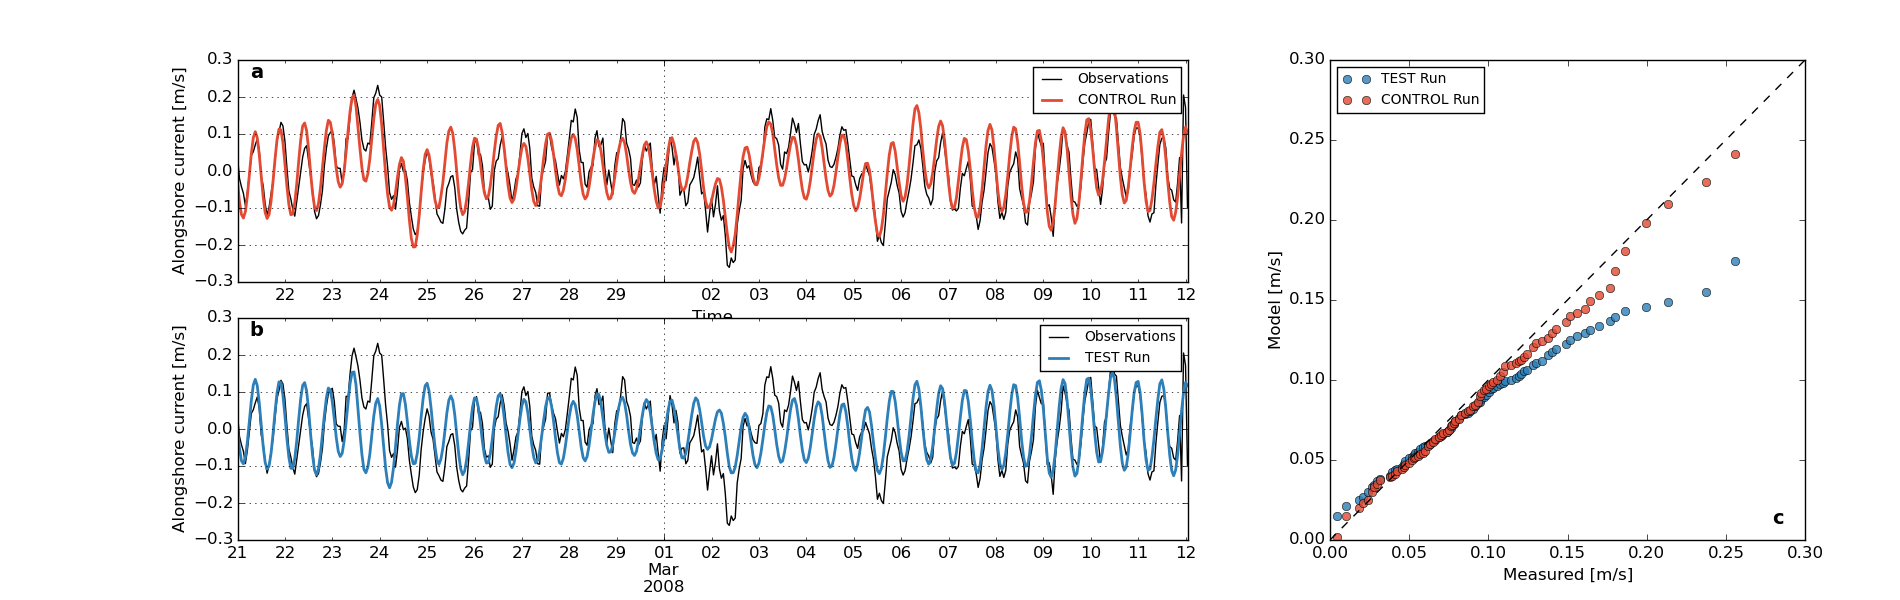
\includegraphics[width=0.73\linewidth]{validation.png}
    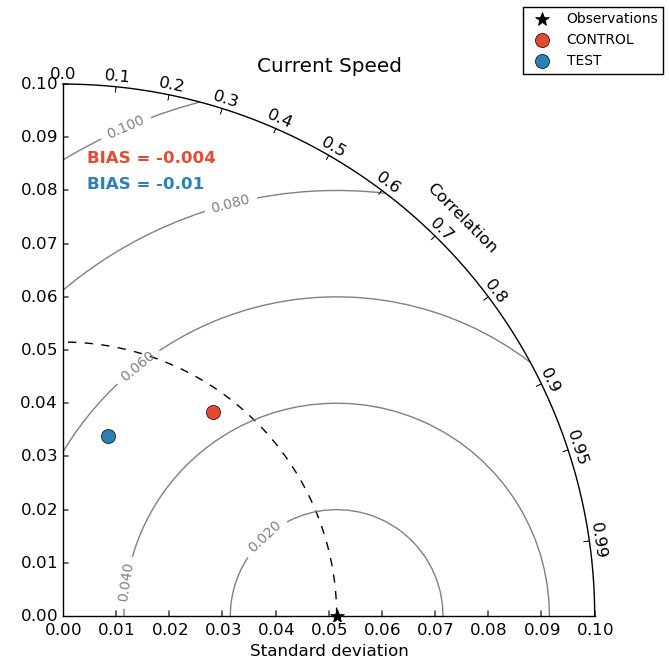
\includegraphics[width=0.27\linewidth]{taylor.png}
    \caption{\label{validation} Comparison of the CONTROL and TEST experiments with {\it in situ} depth-averaged current measurements.}
    \end{figure}

    % \end{block}
%----------------------------------------------------------------------------------------


\end{column} % End of the second column

\begin{column}{\sepwid}\end{column} % Empty spacer column

\begin{column}{\onecolwid} % The third column

    \begin{block}{Plume propagation}

    A passive tracer point source was introduced in both experiments at a constant rate at the surface during 15 days, and than halted and allowed to evolve for 15 additional days. The plume extends over a greater spatial extent on CONTROL, especially in the SE direction. There is also more northward dispersion in CONTROL. The TEST run overestimates concentrations near the source and underestimates at larger distances. 

    \begin{figure}
    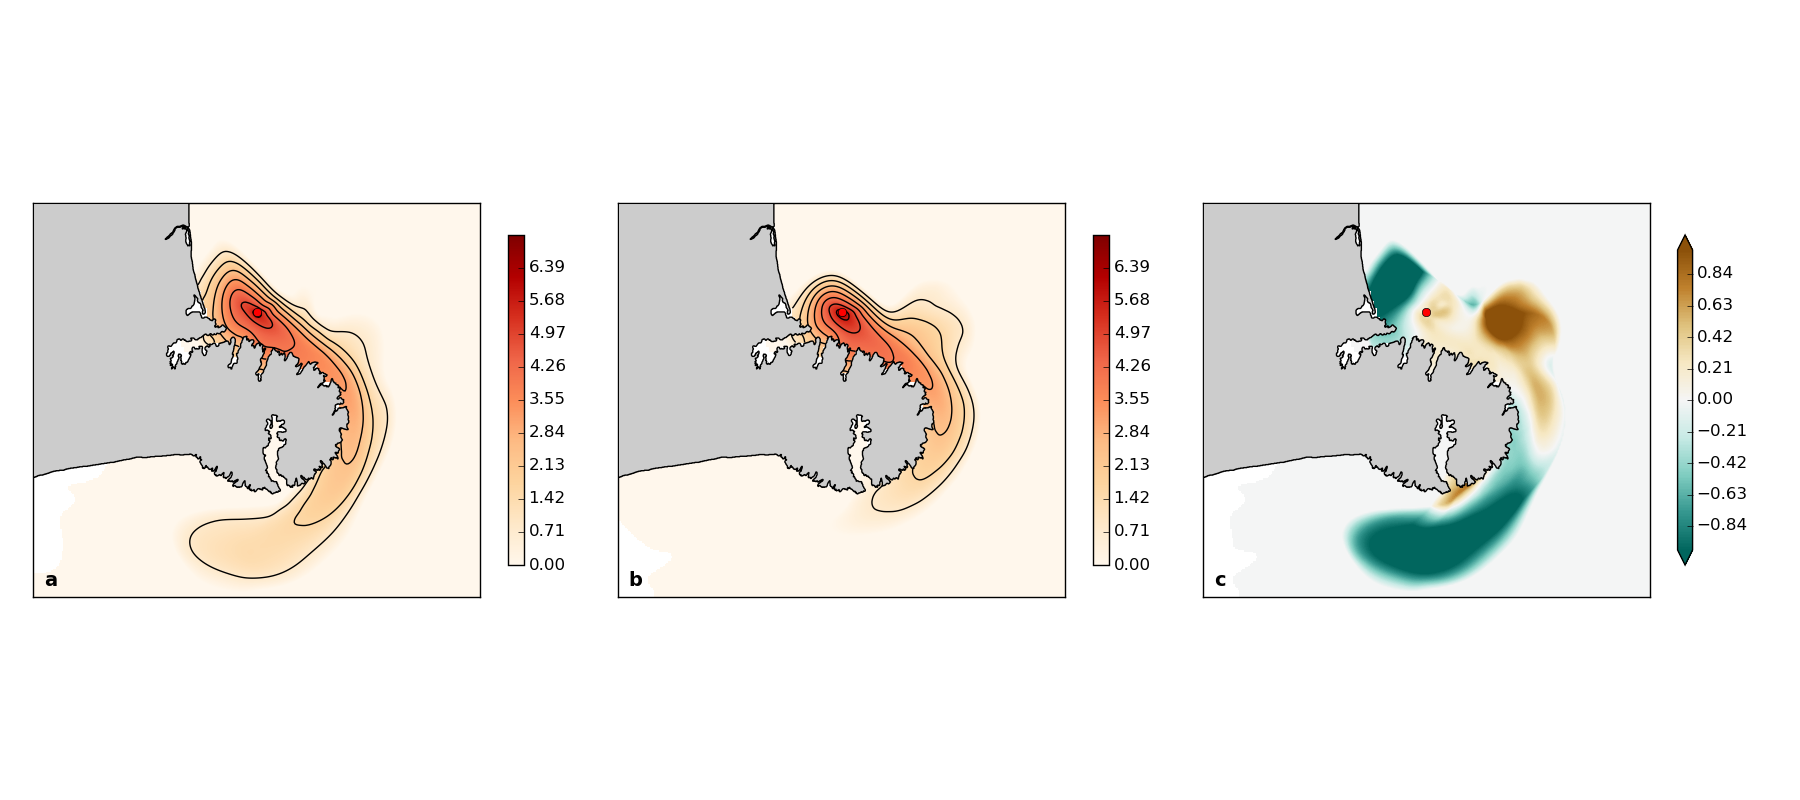
\includegraphics[width=1.0\linewidth]{dye_concentration.png}\\
    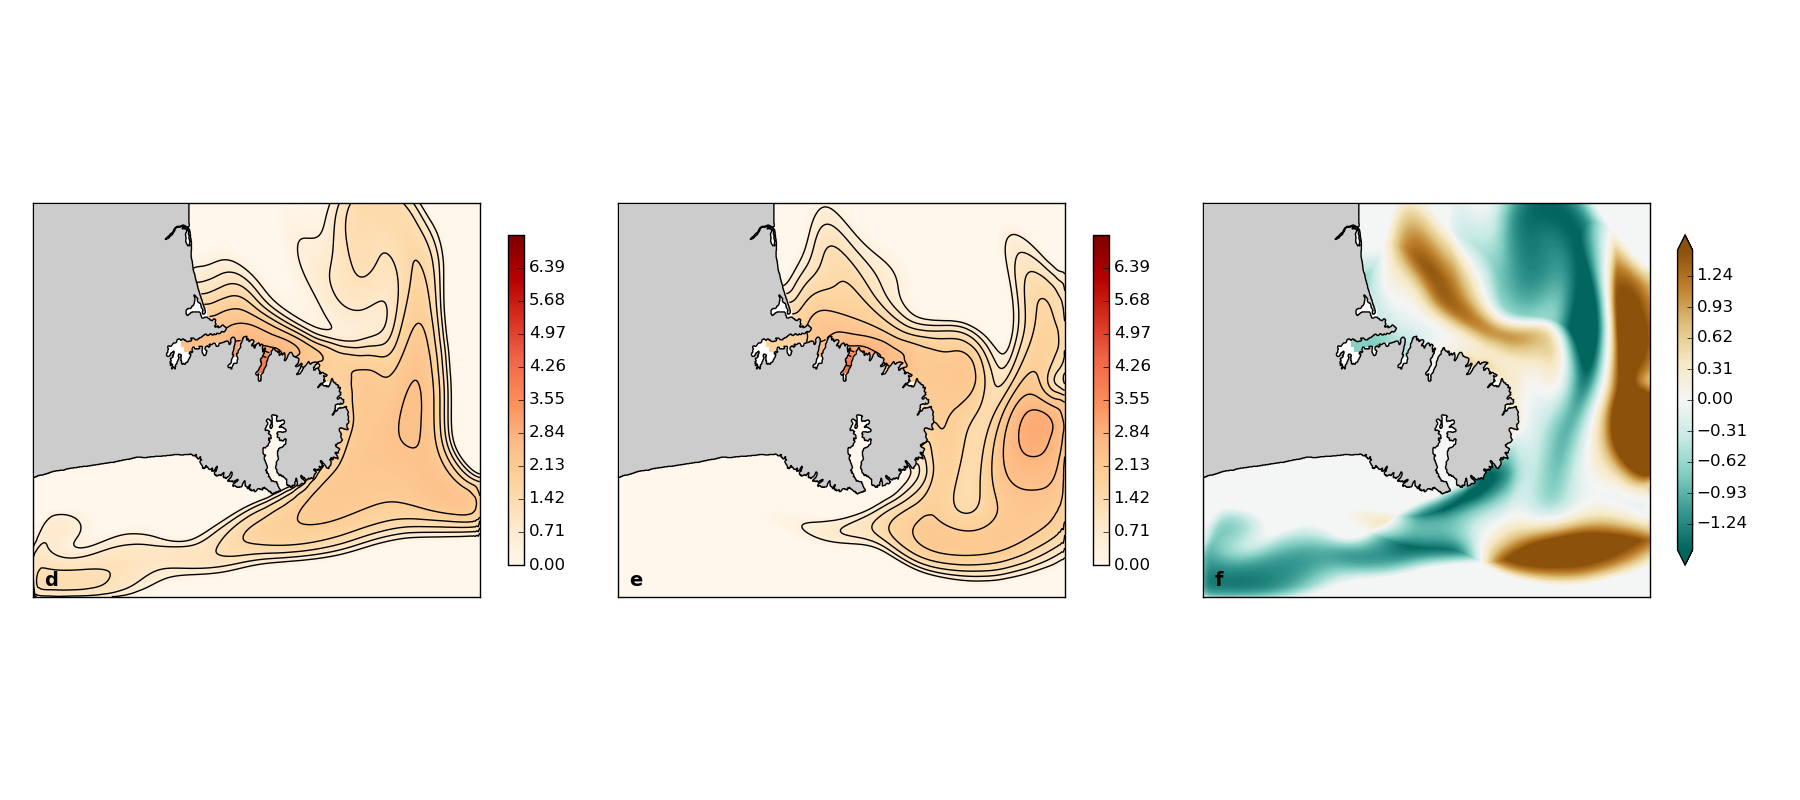
\includegraphics[width=1.0\linewidth]{dye_concentration_last-day.png}
    \caption{\label{dye} (a,b): First 15 day average tracer concentration. (d,e): Daily-averaged tracer concentration 15 days after source halt. (c,f): [TEST - CONTROL] for each case. }
    \end{figure}

    \end{block}

    \setbeamercolor{block alerted title}{fg=black,bg=norange} % Change the alert block title colors

    \begin{alertblock}{Conclusions}

    \begin{small}
    \begin{enumerate}
    \item The SC has a substantial influence in the circulation at PB, accounting for more than half of the total currents at times and controling most of its variability.
    \item The absence of proper open ocean forcing greatly affects model performance for this particular area.
    \item Underestimating the SC implies in less efficient dispersion of passive tracer plumes at the PB inner shelf. 
    \end{enumerate}
    \end{small}

    \end{alertblock}

    %----------------------------------------------------------------------------------------
    %   ADDITIONAL INFORMATION
    %----------------------------------------------------------------------------------------

    % \begin{block}{Additional Information}

    % Maecenas ultricies feugiat velit non mattis. Fusce tempus arcu id ligula varius dictum. 
    % \begin{itemize}
    % \item Curabitur pellentesque dignissim
    % \item Eu facilisis est tempus quis
    % \item Duis porta consequat lorem
    % \end{itemize}

    % \end{block}

    %----------------------------------------------------------------------------------------
    %   REFERENCES
    %----------------------------------------------------------------------------------------

    % \begin{block}{References}

    % \nocite{*} % Insert publications even if they are not cited in the poster
    % \small{\bibliographystyle{unsrt}
    % \bibliography{sample}\vspace{0.75in}}

    % \end{block}

    %----------------------------------------------------------------------------------------
    %   ACKNOWLEDGEMENTS
    %----------------------------------------------------------------------------------------

    \setbeamercolor{block title}{fg=red,bg=white} % Change the block title color

    \begin{block}{Acknowledgements}

    \small{We thank the Lyttelton Port of Christchurch for making the measurements available and the ROMS scientific community. } \\

    \end{block}

    %----------------------------------------------------------------------------------------
    %   CONTACT INFORMATION
    %----------------------------------------------------------------------------------------

    \setbeamercolor{block alerted title}{fg=black,bg=norange} % Change the alert block title colors
    \setbeamercolor{block alerted body}{fg=black,bg=white} % Change the alert block body colors

    \begin{block}{Contact Information}

    \begin{small}
    \begin{itemize}
    \item \href{http://www.metoceanview.com}{http://www.metoceanview.com}
    \item \href{http://www.rsoutelino.com}{http://www.rsoutelino.com}
    \item Email: \href{mailto:r.soutelino@metocean.co.nz}{r.soutelino@metocean.co.nz}
    \end{itemize}
    \end{small}

    \end{block}

    \vspace{3.2cm}

    \begin{center}
    % \begin{tabular}{ccc}
    
\includegraphics[width=0.7\linewidth]{msllogo.jpg}
    % \end{tabular}
    \end{center}

    %----------------------------------------------------------------------------------------

\end{column} % End of the third column

\end{columns} % End of all the columns in the poster

\end{frame} % End of the enclosing frame

\end{document}
